\documentclass[a4paper,11pt] {article}
\usepackage[spanish]{babel}
\usepackage[utf8]{inputenc}
\usepackage{caratula}
\usepackage{a4wide}
%\usepackage{graphicx}
% \usepackage{dot2texi}
% \usepackage{graphs}

\begin{document}

\titulo{Trabajo Pr\'actico Nro. 1}
\fecha{21/04/2010}
\materia{Ingenier\'ia de Software I}
\grupo{}
\integrante{Dinota, Mat\'ias}{076/07}{matiasgd@gmail.com}
\integrante{Frid, Igal Pablo}{231/07}{ipfrid@gmail.com}
\integrante{Huel, Federico Ariel}{329/07}{federico.huel@gmail.com}
\integrante{Leveroni, Luciano}{360/07}{lucianolev@gmail.com}
\integrante{Mosteiro, Agust\'in}{125/07}{agustinmosteiro@gmail.com}

\maketitle

\bigskip

\section*{Introducci\'on}

El objetivo del siguiente trabajo es modelar un sistema para una cadena de pizzer\'ias, denominada Pizza Hack. Con este fin, se utilizar\'an t\'ecnicas de ingenier\'ia de requerimientos, a saber: Diagrama de Contexto y de Objetivos. A su vez, se incluyen en el presente trabajo las explicaciones y detalles de cada uno de los diagramas para clarificar lo expuesto de forma gr\'afica en dichos diagramas. 

El sistema a modelar pretende resolver las necesidades y problemas de una cadena de pizzer\'ias t\'ipica, en la que cada uno de los locales atiende al p\'ublico a trav\'es de un mostrador, es decir, no ofrece la posibilidad de consumir las pizzas en el mismo local. Adem\'as, cabe aclarar que la cadena de pizzer\'ias desea mantener el mismo men\'u en todos sus locales, por lo que un cambio en el men\'u de un local deber\'a verse reflejado en la cartilla de los restantes. Tambi\'en se debe mencionar que en caso de que alg\'un pedido no se pueda preparar en el local donde se encuentra el cliente, se ofrecer\'a derivar su pedido a otro local de la cadena. Por \'ultimo, hay que tener en cuenta que el sistema no debe tener un servidor centralizado para la coordinaci\'on entre locales.

Por medio de la aplicaci\'on de las t\'ecnicas de inginier\'ia de requerimientos se busca explorar distintas opciones para modelar el sistema deseado por la cadena de pizzas. Finalmente, se estudiar\'an las ventajas y desventajas que conlleva elegir cada una de estas alternativas en los aspectos que consideramos relevantes para el funcionamiento del sistema y el beneficio de la cadena de pizzas.  

\section*{Presunciones}

Para la confecci\'on del trabajo, se hicieron las siguientes presunciones:

\begin{itemize}
    \item Pizza Hack no brinda servicio de delivery ni tampoco brinda la posibilidad de comer en el local.
    \item La m\'aquina no contempla manejo de dinero.
    \item Los cambios s\'olo podr\'an proponerse al finalizar el d\'ia, es decir cuando todos los locales ya se encuentren cerrados, para asegurarse de que dicho cambio no genere imprevistos en el men\'u cuando el local est\'a operando.
		\item Cuando un local propone un cambio, debe hacerlo durante su turno, es decir hay un sistema de turnos para proponer cambios entre locales.
		\item El supermercado al que se realizan las compras de los productos para preparar los pedidos posee un sistema de delivery.
\end{itemize}

\section*{Vistas}

\subsection*{Diagramas de objetivos}

En la siguiente secci\'on se presentar\'an los gr\'aficos correspondientes a los diagramas de objetivos referentes al sistema: 

\subsubsection*{Administrar Stock}
\begin{center}
 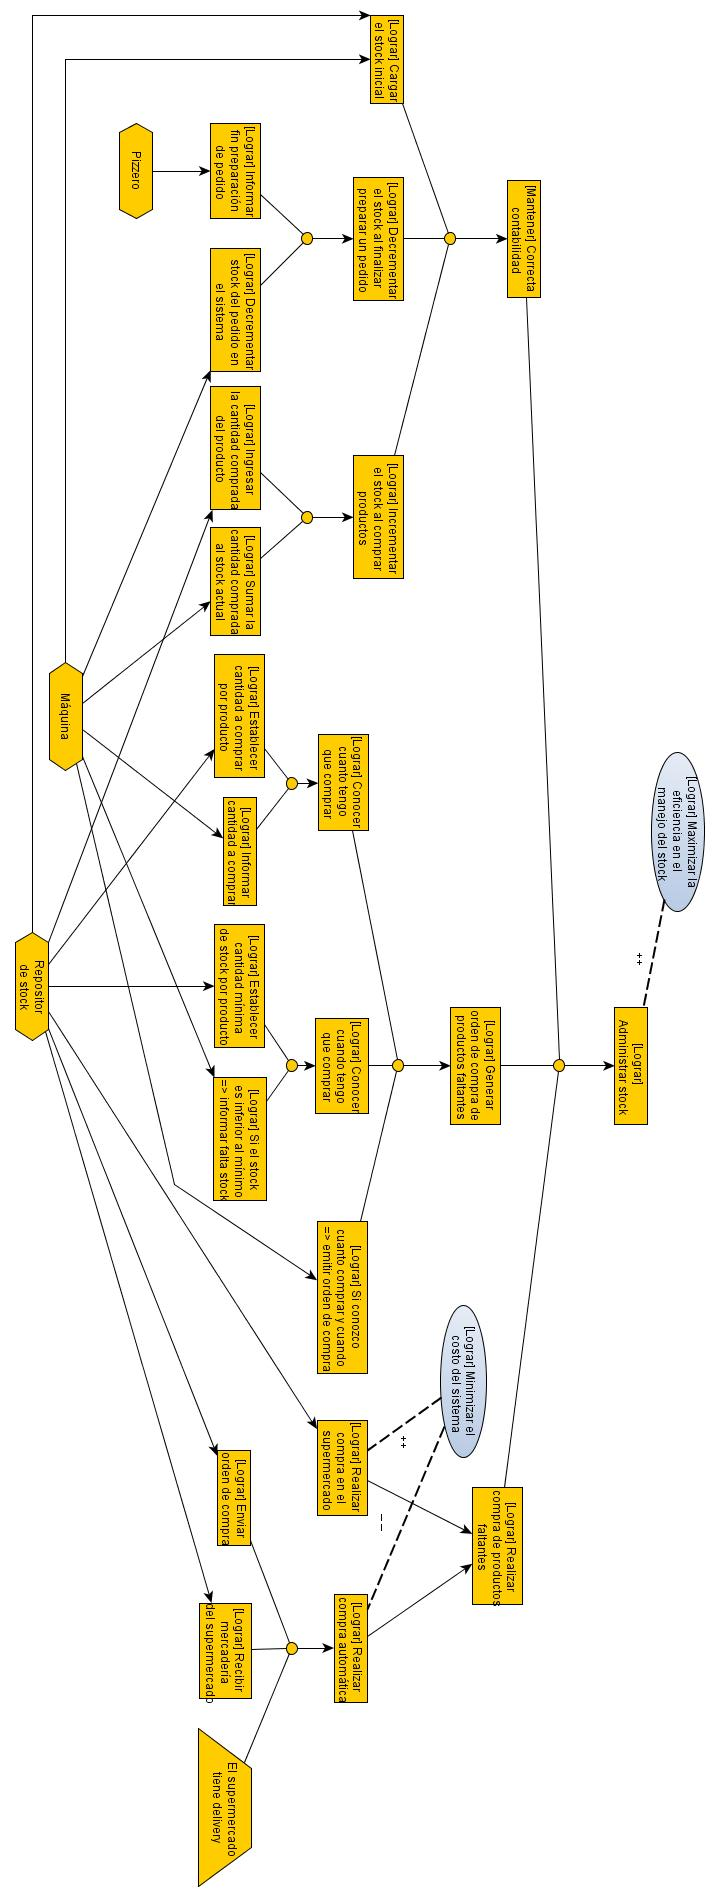
\includegraphics[height=24cm,width=17cm]{Diagramas/AdministrarStock.jpg}
\end{center}

\subsubsection*{Men\'u estandatizado}
\begin{center}
 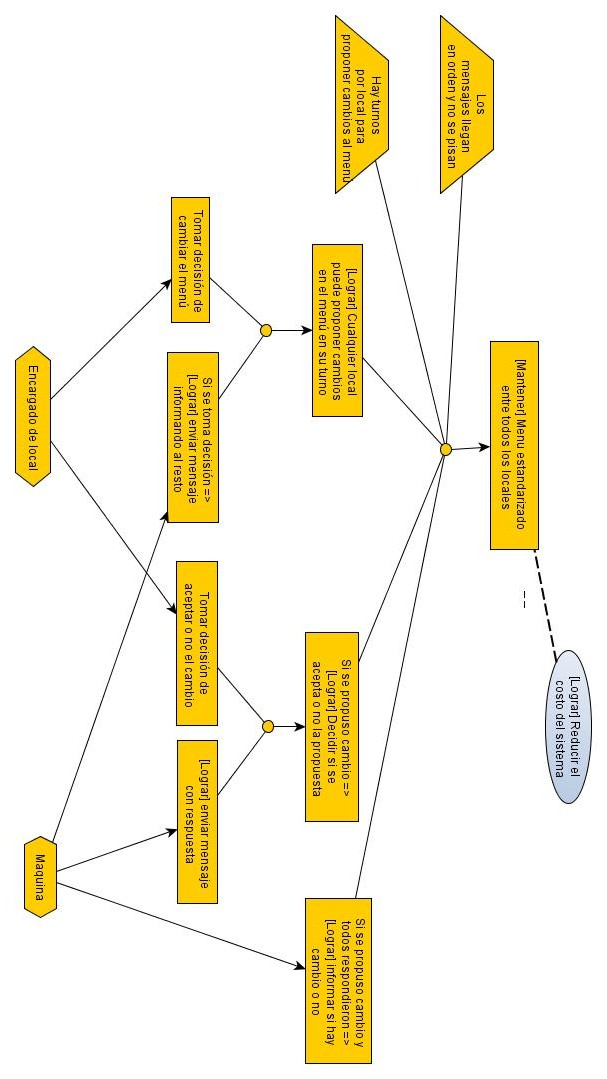
\includegraphics[height=22cm,width=15cm]{Diagramas/MenuEstandarizado.jpg}
\end{center}

\subsubsection*{Tomar pedidos}
\begin{center}
 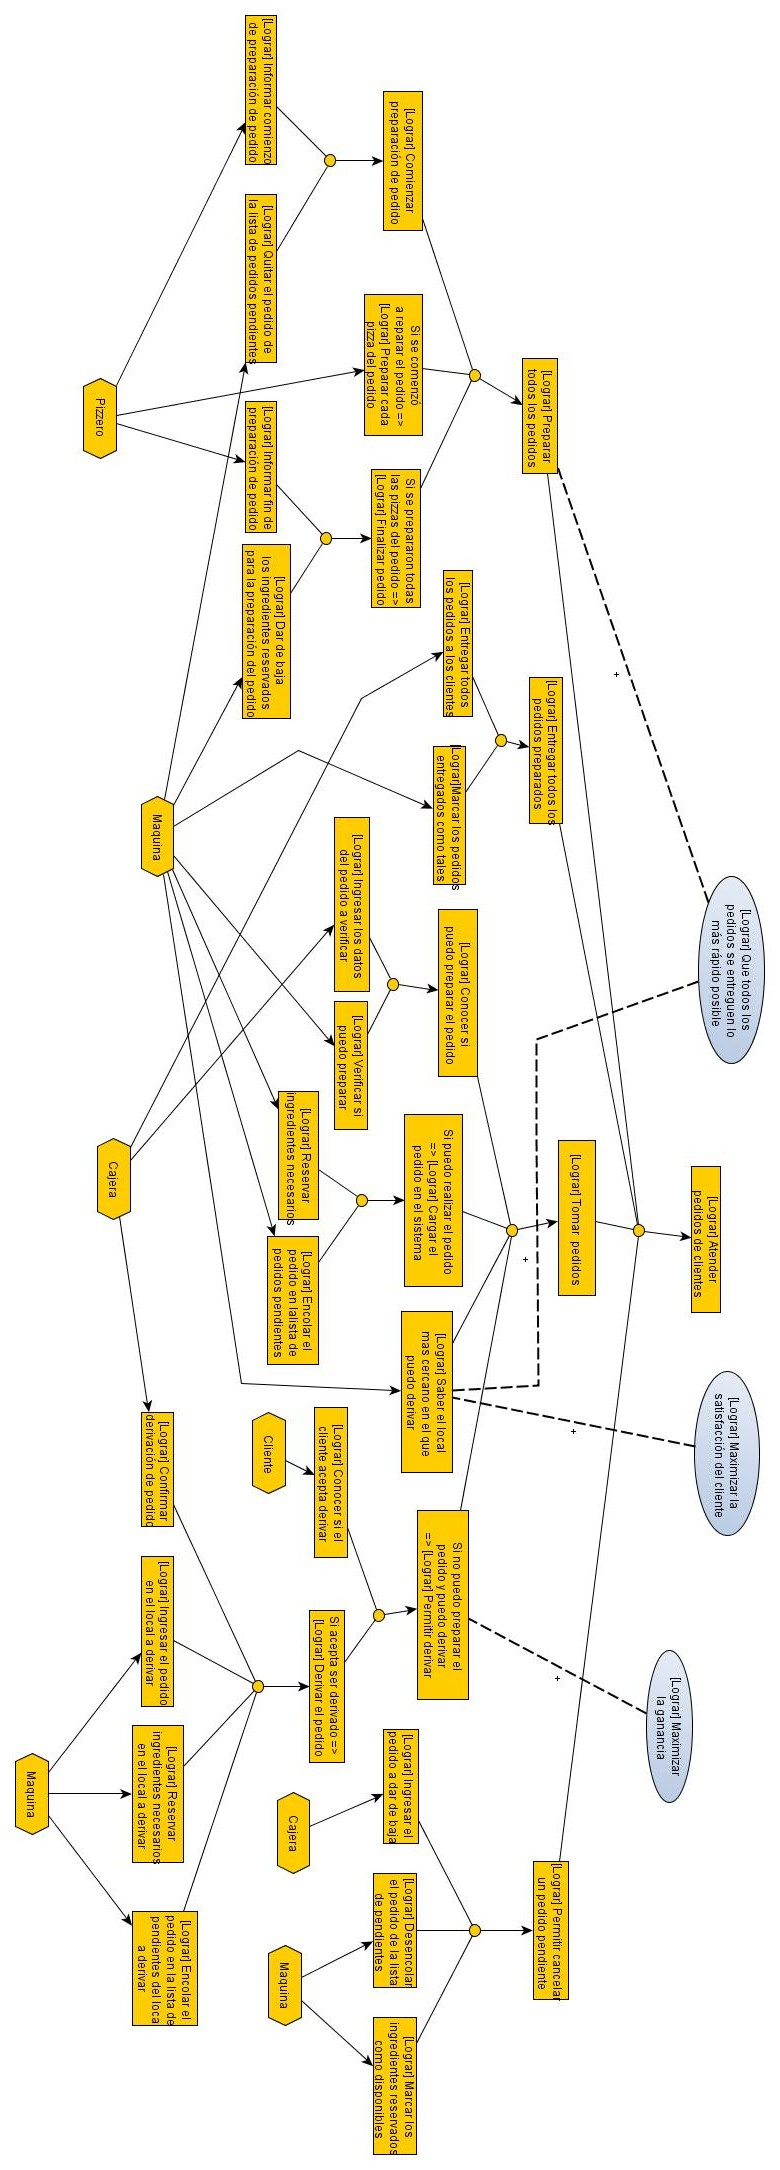
\includegraphics[height=22cm,width=15cm]{Diagramas/TomarPedido.jpg}
\end{center}

\subsection*{Explicaciones}

\subsubsection*{Diagrama: Administrar stock}

\begin{itemize}
\item
Objetivo: Mantener correcta contabilidad.

Definici\'on: Significa que en todo momento se desea conocer el stock disponible.

\item
Objetivo: Lograr cargar stock inicial.

Definici\'on: Cuando se abre un local, es el repositor de stock quien se encarga de ralizar una carga inicial de stock.

\item
Objetivo: Lograr decrementar el stock al finaliar de preparar un pedido.

Definici\'on: El stock se descuenta una vez que el pedido se termina de preparar. Esto se realiza luego de que el pizzero informa que termin\'o de preparar un pedido.

\item
Objetivo: Lograr incrementar el stock al comprar productos.

Definici\'on: Una vez que el repositor de stock compr\'o los productos necesarios, tiene que cargar en el sistema la cantidad comprada de cada producto para poder registrar el nuevo stock.

\item
Objetivo: Lograr conocer cu\'anto tengo que comprar.

Definici\'on: Este objetivo permite automatizar la realizaci\'on de una \'orden de compra de productos. Simplemente se busca en el sistema cu\'al es la cantidad predeterminada a comprar de cierto producto.

\item
Objetivo: Lograr establecer cantidad a comprar por producto.

Definici\'on: El repositor de stock es el encargado de establecer una cantidad predeterminada a comprar de un producto. Este valor puede ir cambiando de seg\'un las necesidades del local.

\item
Objetivo: Lograr conocer cu\'ando tengo que comprar.

Definici\'on: Una vez que el stock de un producto atravieza la cota m\'inima de stock del producto, el sistema dispara una alarma para informar que se debe realizar una compra sobre ese producto ya que est\'a pr\'oximo a agotarse.

\item
Objetivo: Lograr establecer cantidad m\'inima de stock por producto.

Definici\'on: El repositor de stock es el encargado de establecer la cota m\'inima de stock aceptable antes de tener que ir a reponer. Este valor puede ir cambiando de seg\'un las necesidades del local.

\item
Objetivo: Si conozco cu\'anto comprar y cu\'ando comprar => Lograr emitir \'orden de compra.

Definici\'on: Una vez que el sistema dispara la alarma por falta de stock (cu\'ando comprar) y obteniendo la cantidad predeterminada a comprar de un producto (cu\'anto comprar), el sistema emitir\'a una \'orden de compra para ese producto con la cantidad predeterminada especificada.

\item
Objetivo: Lograr realizar compra en el supermercado.

Definici\'on: El repositor de stock se dirige el mismo a realizar las compras de productos faltantes con la \'orden de compra emitida por el sistema.

\item
Objetivo: Lograr realizar compra autom\'atica.

Definici\'on: El repositor de stock env\'ia la \'orden de compra emitida por el sistema al supermercado para que el mismo se encargue de enviar la mercader\'ia.

\item
Objetivo: Lograr recibir mercader\'ia del supermercado.

Definici\'on: El repositor de stock es qui\'en debe aguardar por el pedido realizado al supermercado.

\end{itemize}


\subsubsection*{Diagrama: Men\'u estandarizado entre todos los locales}
\begin{itemize}
 \item 
Objetivo: Mantener Men\'u estandarizado entre todos los locales

Definici\'on: Los encargados de los locales deber\'an poder proponer una modificaci\'on, agregado o remoci\'on de cualquier producto del men\'u actual. Este cambio deber\'a ser aceptado por los dem\'as locales para lograr que el mismo se haga efectivo. Con este prop\'osito, el sistema deber\'a ser capaz de informar el cambio que desea hacerse a los dem\'as locales para que estos puedan decidir su aceptaci\'on o rechazo. Una vez que todos los locales responden, se toma una decisi\'on en base a dichas respuestas. El cambio s\'olo es aceptado si la decisi\'on de todos los locales es afirmativa.

\item 
Objetivo: Lograr Cualquier local puede proponer cambios en el men\'u en su turno

Definici\'on: Una vez que un local posea el turno para realizar una propuesta de cambio en el men\'u, el sistema debe brindar la posibilidad de efectuar un cambio, ya sea un agregar, quitar o modificar alg\'un producto de la cadena de pizzas.

\item 
Objetivo: Si se toma decisi\'on =$>$ Lograr enviar mensaje al resto

Definici\'on: Cuando el encargado de un local decide proponer un cambio en el men\'u, el sistema deber\'a ser capaz de enviar un mensaje a los demás locales notificando el cambio que se propone.

\item 
Objetivo: Si se propuso cambio =$>$ Decidir si se acepta o no la propuesta

Definici\'on: Si un local propuso un cambi\'o, se recibir\'a un mensaje pidiendo la confirmaci\'on o el rechazo del mismo. El encargado debe tomar esta decisi\'on y el sistema deber\'a ser capaz de enviar su respuesta al local que propuso dicha modificaci\'on del men\'u.

\item 
Objetivo: Lograr enviar mensaje con respuesta

Definici\'on: Se debe lograr enviar un mensaje con la respuesta al cambio de men\'u.

\item 
Objetivo: Si se propuso cambio y todos respondieron =$>$ lograr informar si hay cambio o no

Definici\'on: Si se recibe la respuesta de todos los locales al cambio propuesto, se debe lograr enviar un mensaje de confirmaci\'on o rechazo del cambio, a trav\'es de un correo electrónico, a todos los locales para que se pueda actualizar el men\'u en cada uno de los locales. Si un local no llegara a responder al cambio de men\'u propuesto en el lapso de tres horas se considera que la respuesta de dicho local fue afirmativa.

\end{itemize}

\subsubsection*{Diagrama: Tomar pedidos}
\begin{itemize}
 \item 
Objetivo: Lograr preparar todos los pedidos

Definici\'on: Significa que deben prepararse todos los pedidos que se hayan efectuado en ese local sin dejar ninguno incompleto.

\item 
Objetivo: Comenzar preparaci\'on de pedido

Definici\'on: Una vez que el pizzero le informa al sistema que comenzar\'a con la preparaci\'on de un pedido pendiente, dicho pedido deja de estar pendiente y pasa a estar en estado de \textit{En proceso}.

\item 
Objetivo: Si se prepararon todas las pizzas del pedido =$>$ lograr finalizar pedido

Definici\'on: El pizzero debe preparar cada una de las pizzas del pedido para reci\'en ah\'i poder marcar el pedido como finalizado. Una vez que se terminen de preparar todas las pizzas, el pizzero le informa al sistema que termin\'o de preparar el pedido. Una vez hecho esto el sistema le cambia el estado al pedido a \textit{Finalizado} y se decrementa el stock reservado para el pedido que ya fue utilizado en la preparaci\'on del mismo.

\item 
Objetivo: Lograr entregar todos los pedidos a los clientes

Definici\'on: Una vez que el pedido se encuentra en estado \textit{Finalizado}, el mismo debe ser entregado al cliente y luego ponerlo en estado Entregado.

\item 
Objetivo: Lograr conocer si puedo preparar el pedido.

Definici\'on: Para saber si puedo preparar un pedido o no dentro de un local se debe primero ingresar el pedido y luego el sistema chequea si tiene stock disponible o no para su preparaci\'on e informa a la cajera.

\item 
Objetivo: Si puedo preparar el pedido =$>$ lograr cargar el pedido en el sistema

Definici\'on: Si el local posee stock para preparar un pedido, debe poder cargarse el mismo en el sistema. Una vez que el pedido se carga, se reservan autom\'aticamente todos los ingredientes necesarios para su reparaci\'on para garantizar su entrega.

\item 
Objetivo: Lograr saber el local mas cercano en el que puedo derivar.

Definici\'on: Para cumplir con este objetivo, el sistema realiza una comunicaci\'on con sus locales m\'as cercanos donde les informa el pedido a preparar. Los locales al recibir la informaci\'on eval\'uan si tienen stock suficiente para satisfacer el pedido, de ser as\'i le informan al local que pueden y si no informan que no. Una vez que el local tiene los datos de sus locales vecinos, tiene la informaci\'on de cu\'al es el local m\'as cercano en el cu\'al se puede derivar un pedido.

\item 
Objetivo: Si no puedo preparar el pedido y puedo derivar =$>$ lograr permitir derivar el pedido.

Definici\'on: Una vez que conozco el local m\'as cercano a derivar, se le consulta al cliente si desea derivar el pedido a otro local y retirarlo ah\'i. Si el cliente afirma se realiza el pedido en el otro local, lo cual implica la reserva de ingredientes en el otro local para garantizar su preparaci\'on y se ingresa el pedido en la lista de pedidos pendientes del nuevo local.

\item 
Objetivo: Lograr cancepar un pedido pendiente

Definici\'on: S\'olo se pueden cancelar los pedidos que se encuentran pendientes de preparaci\'on, es decir, los pedidos que no se comenzaron a preparar. Esto es para que puedan reutilizarse los ingredientes reservados en caso de una cancelaci\'on.

\end{itemize}

\subsection*{Diagramas de contexto}

En la siguiente secci\'on se presentar\'an los gr\'aficos correspondientes a los diagramas de contexto referentes al sistema. Se mostrar\'an dos diagramas que representan las dos alternativas planteadas en los o-refinamientos del diagrama de objetivos de administraci\'on de stock: 

\begin{center}
 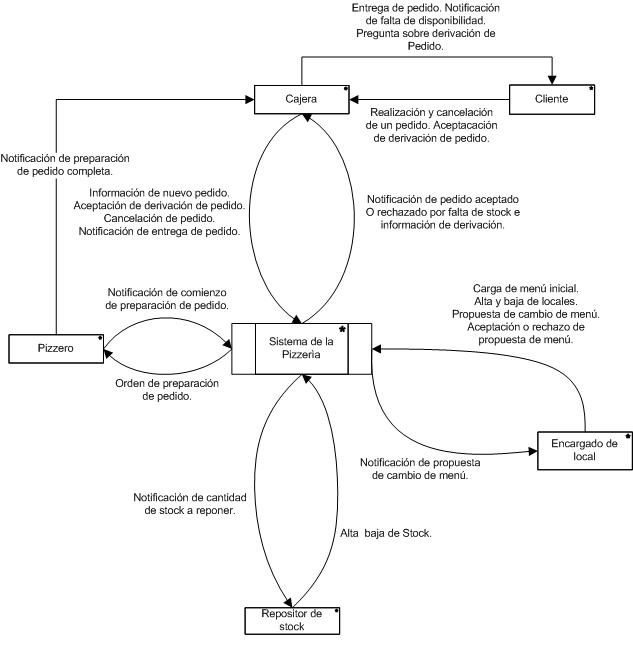
\includegraphics{Diagramas/Diagramadecontexto.jpg}
\end{center}
\begin{center}
 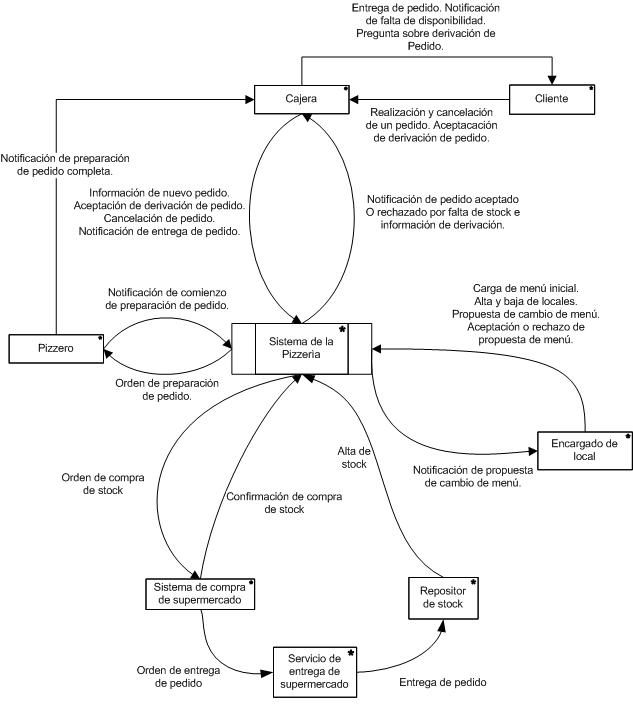
\includegraphics{Diagramas/Diagramadecontextoconstockautomatico.jpg}
\end{center}

\section*{Escenarios}
A continuaci\'on se mostrar\'an algunos de los posibles escenarios que se podr\'ian llegar a presentarse en la cadena de pizzas descripta. 
\begin{itemize}
	\item Un cliente realiza un pedido a la cajera de un local. La cajera ingresa los datos del pedido a verificar y la m\'aquina le informa si puede preparar o no el pedido. El mismo puede ser preparado. La cajera confirma el pedido con el cliente y lo carga en el sistema. En este momento, \'este se almacena junto con los dem\'as pedidos pendientes y se reservan los ingredientes necesarios para su preparaci\'on. Mientras tanto, el pizzero se encuentra preparando distintos pedidos cuando, en un determinado momento, el sistema le informa que el siguiente es el del cliente anteriormente mencionado. Una vez listo el pedido, se le entrega al cliente y \'este se retira.
	\item Un cliente realiza un pedido a la cajera de un local. La cajera ingresa los datos del pedido a verificar y la m\'aquina le informa si puede preparar o no el pedido. El mismo no puede ser preparado. El sistema le informa a la cajera el local m\'as cercano donde se puede preparar dicho pedido. Se le ofrece al cliente la opci\'on de derivar su pedido a ese local y \'este acepta. La cajera deriva el pedido reservandose los ingredientes necesarios en el otro local donde el cliente lo retira posteriormente.
	\item Al pizzero se le cae una de las pizzas al suelo. En ese instante, informa al encargado lo ocurrido y el mismo da de baja el stock correspondiente. A continuaci\'on, el pizzero vuelve a realizar la pizza.
    \item Luego de realizar el pedido, el cliente se arrepiente y decide cancelarlo. En este caso, la cajera ingresa dicha cancelaci\'on en el sistema retirando el pedido de la lista de pedidos pendientes. Si la pizza no se comenz\'o a preparar, los ingredientes reservados para dicho pedido estan disponibles para ser utilizados en alg\'un otro. Si la pizza ya fue preparada o se encuentra en preparaci\'on, los ingredientes se pierden.
\end{itemize}

\section*{Discusi\'on}

En primer lugar, se procedi\'o a la construcci\'on de un diagrama de objetivos para comenzar a pensar sobre los aspectos importantes del sistema. Por cuestiones de claridad, analizaremos las discusiones referentes a la construcci\'on de cada parte de este diagrama por separado.

En lo referente a los asuntos del manejo de stock, como primera idea se pens\'o en la soluci\'on cl\'asica contar con un agente (Repositor de stock) encargado de solucionar cada inconveniente del tema. Luego, se pens\'o en hacer uso de la m\'aquina para poder contar con un registro del stock disponible de manera tal que el repositor solamente monitoree peri\'odicamente el equipo para realizar las compras necesarias. En este \'ambito se present\'o la posibilidad t\'ipica en la que el repositor realiza las compras por su cuenta en cualquier mercado y adem\'as surgi\'o la idea de hacer dichas compras a trav\'es del sistema de delivery del supermercado. Este \'ultimo caso aumenta la complejidad del sistema, que tendr\'ia que ser capaz de comunicarse con el sistema de entregas del supermercado, por lo que aumentar\'ia tambi\'en el costo del sistema en consecuencia.

Otro aspecto interesante del sistema consisti\'o en permitir la modificacion del men\'u de la cadena por parte de los locales. A partir de este evento, surgio un tema que result\'o ser central en el dise\~no del sistema. Para mantener la consistencia del mismo, al realizar cambios en el men\'u, era necesario informar al resto de los locales de tal cambio ya que el sistema a realizar ser\'a de tipo distribuido. Esto oblig\'o a pensar fuertemente sobre este aspecto. Como primera opcion, se pens\'o en asignar un local central encargado de tomar las decisiones con respecto a dichos cambios. Sin embargo, esto chocaba con parte de lo requerido para el sistema ya que no todos los locales podr\'ian proponer cambios al men\'u. Finalmente, se decidi\'o por realizar un sistema basado en una comunicaci\'on descentralizada entre los locales. Cada local dispone de un turno o intervalo de tiempo en el que puede proponer los cambios que considera necesarios en el men\'u. Es decir, si un local decide hacer un cambio y es su turno, el sistema enviar\'a mensajes a los dem\'as locales para que estos confirmen o rechacen dicha modificaci\'on.
 
Uno de los aspectos m\'as importantes a analizar fue la atenci\'on del cliente. En primer lugar, se trat\'o el tema relacionado con la derivaci\'on de clientes a otros locales. Esta caracter\'istica del sistema result\'o interesante ya que brinda una posibilidad extra a los clientes de obtener su pedido, maximizando as\'i su satisfacci\'on. Otra manera de lograr esto \'ultimo fue tratar de disminuir el tiempo de espera del cliente en el caso de que el pedido pueda ser preparado en el local. Para cumplir con este requerimiento, se utiliz\'o un algoritmo que optimice el \'orden de preparacion de cada pedido, de manera de poder disminuir el tiempo global de realizaci\'on de los pedidos.

A pesar de todas estas consideraciones, como en todo sistema, existen casos para los cuales el sistema no presenta una soluci\'on. Entre ellos, se encuentra el caso en que, durante la preparaci\'on de un pedido, el pizzero comete un error que arruina la preparaci\'on, desperdiciando los ingredientes correspondientes. El problema aparece cuando el local no cuenta con reservas de stock para preparar la pizza nuevamente. Otro problema relacionado con la p\'erdida de stock ocurre cuando, en caso de contar con el sistema autom\'atico de compra de stock, el proveedor en cuesti\'on se equivoca al traer los ingredientes.

\section*{Conclusiones}

A la hora de encarar el trabajo pr\'actico se presentaron dos caminos posibles por los cuales comenzar con el dise\~no del sistema. Pudimos haber comenzado realizando el diagrama de contexto, sin embargo se opt\'o por realizar primero el diagrama de objetivos. Esta decisi\'on se tom\'o ya que nos pareci\'o mas intuitivo pensar en objetvos generales del sistema que en acciones puntuales del mismo. Se nos ocurri\'o que a partir de conocer bien cuales eran los distintos objetivos a cumplir se podr\'ian deducir con mayor facilidad los eventos que ocurren en el dominio manteniendo as\'i una trazabilidad entre ambos esquemas.

A pesar de lo mencionado anteriormente, fue durante el desarrollo del diagrama de objetivos donde se presentaron la mayor parte de las dificultades. 

El primer problema con el que nos encontramos fue que una vez terminado el diagrama notamos ciertas inconsistencias y surgieron nuevos objetivos que no hab\'iamos contemplado en primera instancia. Esto produjo una importante p\'erdida de tiempo ya que tuvimos que refactorizar el esquema numerosas veces.

Tambi\'en se presentaron inconvenientes a la hora de distinguir entre objetivos duros y blandos. En la primer etapa del armado del diagrama, por no tener en cuenta esta distinci\'on pensamos a todos los objetivos como duros. R\'apidamente nos dimos cuenta que varios de ellos en realidad deb\'ian ser considerados como blandos ya que cuadraban m\'as con este tipo de objetivo.

Como conclusi\'on final del trabajo pudimos observar que si bien en una primera instancia el sistema a modelar parec\'ia sencillo, luego de analizarlo con mayor profundidad notamos que su complejidad era mayor a la esperada. De no haber hecho este an\'alisis, los distintos problemas que se presentaron durante el modelaje hubieran representado un costo mucho mayor en etapas posteriores. Es por esto que nos pareci\'o realmente importante realizar una ingenier\'ia de requerimientos a la hora de encarar el desarrollo de un sistema.

\end{document}